\subsubsection{In-System-Programmer}
\label{subsubsec:insystemprogrammer}

\begin{minipage}[b][6.5cm][t]{0.5\textwidth}
Als ISP wird der AVR Dragon von Atmel verwendet. Dieser ist ein kostengünstiges Entwicklungstool, welches alle Programmiermodi für die Atmel AVR-Device Familien (z.B. der verwendete atmega2560 Mikrocontroller, siehe \textbf{Referenz}) unterstützt. Er enthält auch eine vollständige Debugging-Unterstützung für die meisten AVR-Devices. Diese wurde aber in diesem Projekt nicht genutzt. Der AVR Dragon wird über das USB 2.0 Kabel (Typ B) gespiesen, mit welchem er an den Computer angeschlossen wird. \cite{avrdragonug}\\

\end{minipage}
\begin{minipage}[b][6.5cm][t]{0.48\textwidth}
\centering
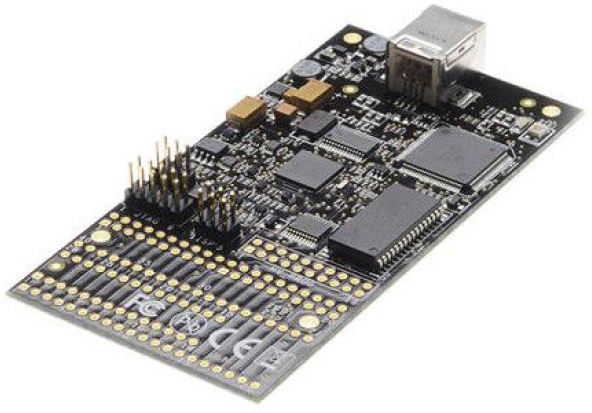
\includegraphics[width=\textwidth]{graphics/ISP/avr_dragon.PNG}
\captionof{figure}{AVR Dragon \cite{avrdragonug}}
\end{minipage}

\paragraph{Programmierinterface}
\label{para:programmierinterface}

Der AVR Dragon kann direkt mit dem Target Board, also der Wetterstation verbunden werden. Dafür werden vom AVR Dragon verschiedene Programmierinterfaces unterstützt: \cite{avrdragonug}\\

\begin{itemize}
	\item SPI Programming 
	\item High Voltage Serial Programming
	\item Parallel Programming
	\item JTAG Programming (\textit{D})
	\item PDI Programming (\textit{D})
	\item aWire Programming (\textit{D})
\end{itemize}
Jene, welche mit einem (\textit{D}) gekennzeichnet sind, dienen auch als Debugging Interface. In Bezug auf das Target Board wird der atmega2560 Mikrocntroller der Wetterstation über das SPI Interface programmiert. Der dafür vorgesehene SPI Header (6-Pin Header) ist auf dem AVR Dragon bereits gemounted, wodurch keine Lötarbeiten erforderlich sind (Abb. \ref{fig:spiheader}, rotes Rechteck).\\

\begin{center}
\begin{minipage}[b][7cm][t]{0.4\textwidth}
\centering
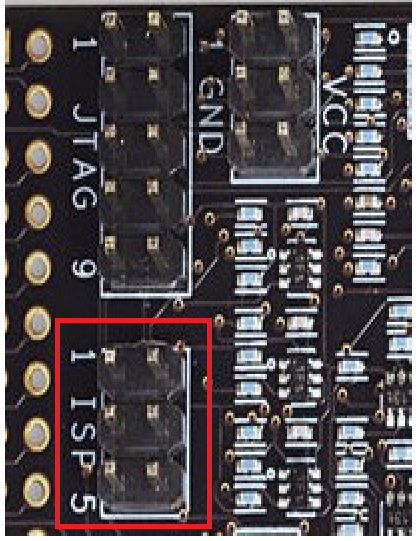
\includegraphics[height=6cm]{graphics/ISP/spi_header.PNG} 
\captionof{figure}{SPI Header \cite{avrdragonug}}
\label{fig:spiheader}
\end{minipage}
\begin{minipage}[b][7cm][t]{0.58\textwidth}
\centering
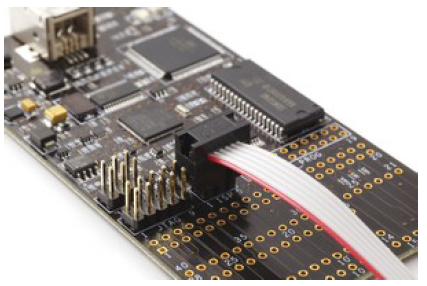
\includegraphics[height=6cm]{graphics/ISP/spi_header_anschluss.PNG} 
\captionof{figure}{Anschluss \cite{avrdragonug}}
\label{fig:spiheader_anschluss}
\end{minipage}
\end{center}

Beim Anschließen des Target Boards sollte darauf geachtet werden, dass die Speisespannung des Targets (3.3V) an dem Pin 2 des Headers angeschlossen ist. Somit kann der AVR Dragon mittels internem Level Converter alle Signale zwischen dem Target Board und sich selbst dem Target anpassen. Das Flachbandkabel sollte also wie in der Abbildung \ref{fig:spiheader_anschluss} angeschlossen werden.

\subparagraph{Zu Beachten:}
Da die $\mu$SD-Karte auf dem Target Board auch über das SPI Interface an den Mikrocontroller angeschlossen ist, so sollten die Jumper beim Anschließen entfernt werden. Es könnte zu Komplikationen führen, wenn Peripherie beim Flash-Vorgang noch an das SPI Interface angeschlossen ist.\\

\paragraph{Device Programming}
\label{para:device_programming}
Um auf das Target (Wetterstation) das Programm flashen zu könenn, müssen noch einige Dinge berücksichtigt werden. In diesem Kapitel wird das wichtigste in Kürze für das Device Programming erklärt. Die folgende Bildabfolge (Abb. \ref:{fig:deviceprogramming} bis \ref{fig:flashing}) soll den Ablauf veranschaulicht erklären und aufzeigen, worauf geachtet werden muss.\\

\todo[inline]{In diesem Kapitel noch auf die Bilder eingehen.}
\begin{figure}[h]
\centering
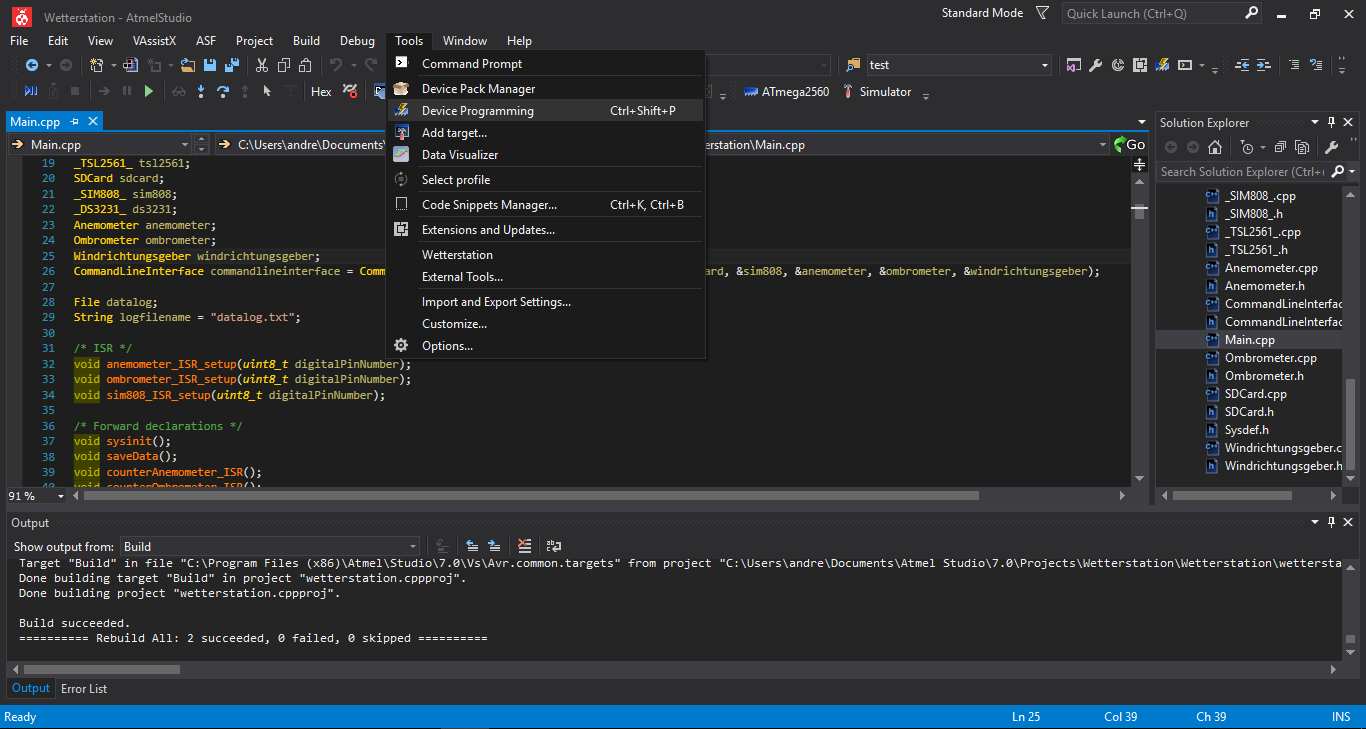
\includegraphics[width=0.7\textwidth]{../../../graphics/device_programming/1.PNG}
\caption{Auswahl Device Programming}
\label{fig:deviceprogramming}
\end{figure}
\begin{figure}[h]
\centering
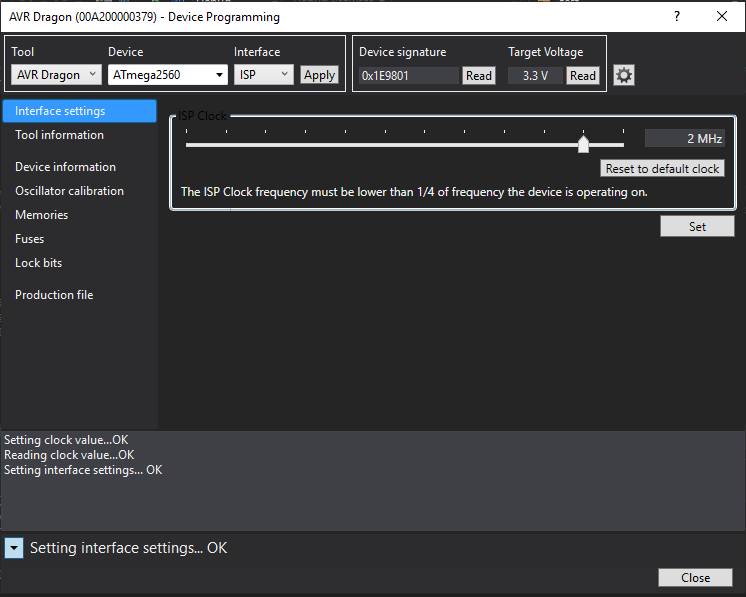
\includegraphics[width=0.7\textwidth]{../../../graphics/device_programming/2.PNG}
\caption{Einstellung des ISP Clocks}
\label{fig:einstellung des ispclocks}
\end{figure}
\begin{figure}[h]
\centering
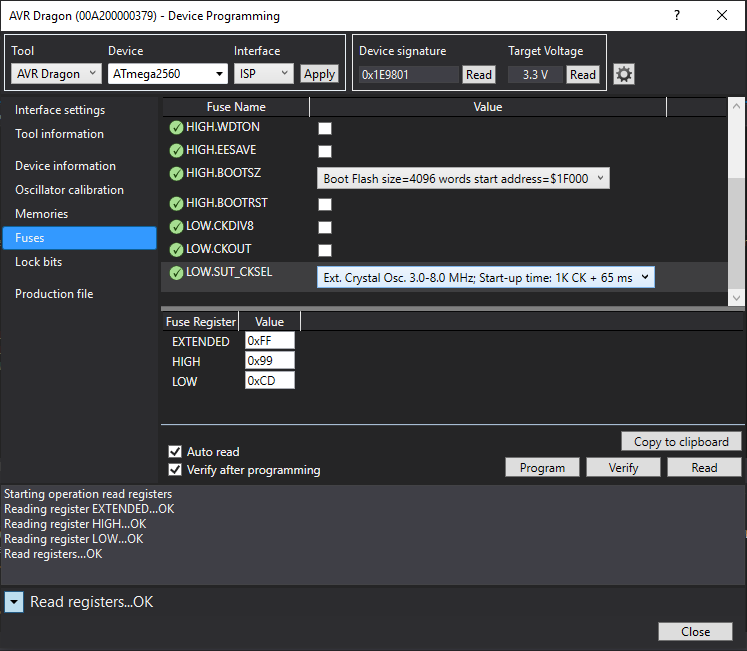
\includegraphics[width=0.7\textwidth]{../../../graphics/device_programming/3.PNG}
\caption{Fuse Register}
\label{fig:fuseregister}
\end{figure}
\begin{figure}[h]
\centering
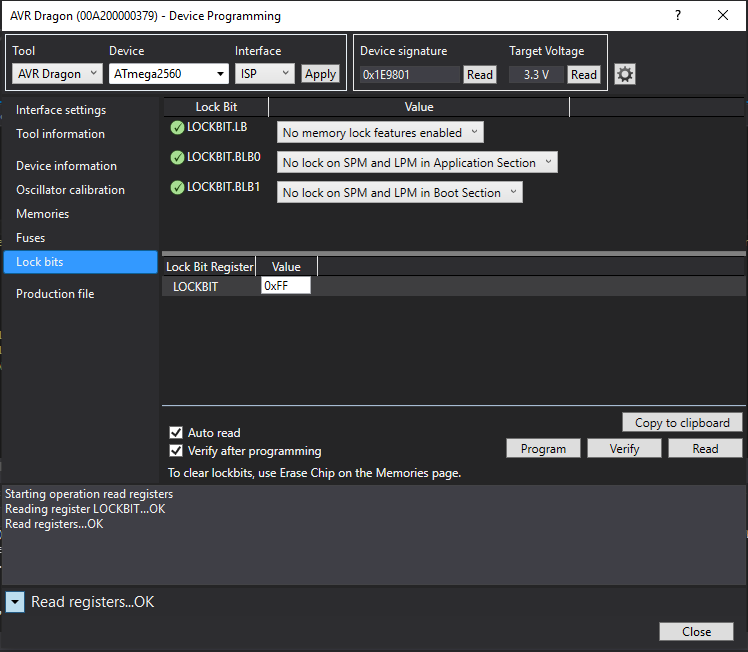
\includegraphics[width=0.7\textwidth]{../../../graphics/device_programming/4.PNG}
\caption{Lock Bits}
\label{fig:lockbits}
\end{figure}
\begin{figure}[h]
\centering
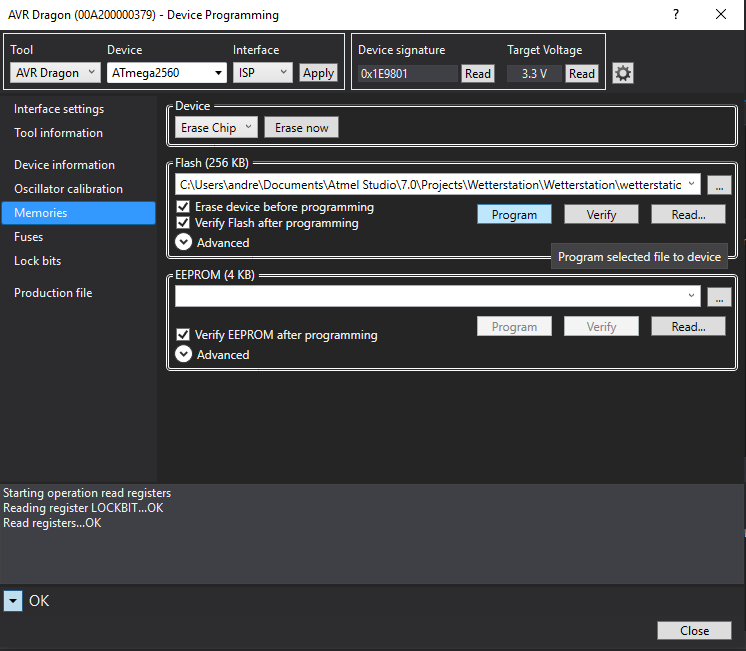
\includegraphics[width=0.7\textwidth]{../../../graphics/device_programming/5.PNG}
\caption{Flashing}
\label{fig:flashing}
\end{figure}
